\section{التحكم منخفض المستوى \LR{Low-Level Control}}



يمثل التحكم منخفض المستوى بالمفاصل \LR{Low-Level Joint Control (LLC)} المرحلة المسؤولة عن توليد إشارات التحكم اللازمة لجعل مفاصل الذراع تتبع المواضع والسرعات المرجعية المطلوبة. في هذه المرحلة لا يتم التركيز على تخطيط المسار العام أو اتخاذ القرار، وإنما على ضمان أن كل مفصل يستجيب بصورة مناسبة للمرجع المعطى له.

يعتمد هذا المستوى من التحكم على النموذج الديناميكي للذراع ونموذج المشغلات من أجل حساب إشارة التحكم المناسبة، سواء كانت جهداً مباشراً أو عزماً يتم تحويله لاحقاً إلى جهد مكافئ. لذلك تم في هذا القسم تطبيق ومقارنة ثلاث خوارزميات تحكم منخفض المستوى، وهي متحكم \LR{PID} مع تعويض الجاذبية، والتحكم التكيفي المعتمد على العزم المحسوب \LR{ACTC}، والتحكم الانزلاقي \LR{SMC}.









%###############################################
%PID
%###############################################



















\subsection{تطبيق متحكم \LR{PID} مع تعويض الجاذبية}
\label{subsec:pid_gravity_compensation}

بعد صياغة النموذج الديناميكي للذراع الروبوتية بصيغة مناسبة للتحكم، تم تطبيق متحكم من نوع \LR{PID} بهدف تتبع مواضع مرجعية محددة لمفاصل الذراع. يعتمد المتحكم على حساب خطأ الموضع وخطأ السرعة لكل مفصل، ثم توليد إشارة تحكم مناسبة يتم إرسالها إلى نموذج المشغلات.

يعرف خطأ الموضع بالعلاقة:

\begin{equation}
e(t)=q_{ref}(t)-q(t)
\label{eq:pid_position_error}
\end{equation}

كما يعرف خطأ السرعة بالعلاقة:

\begin{equation}
\dot{e}(t)=\dot{q}_{ref}(t)-\dot{q}(t)
\label{eq:pid_velocity_error}
\end{equation}

أما الحد التكاملي فيمثل تراكم خطأ الموضع مع الزمن، ويعطى بالعلاقة:

\begin{equation}
e_{int}(t)=\int_0^t e(\tau)\,d\tau
\label{eq:pid_integral_error}
\end{equation}

وبناءً على ذلك، فإن إشارة التحكم الناتجة عن متحكم \LR{PID} تكتب كما يلي:

\begin{equation}
u_{PID}
=
K_p e(t)
+
K_i e_{int}(t)
+
K_d \dot{e}(t)
\label{eq:pid_control_signal}
\end{equation}

حيث تمثل \(K_p\) مصفوفة الكسب التناسبي، وتمثل \(K_i\) مصفوفة الكسب التكاملي، بينما تمثل \(K_d\) مصفوفة الكسب التفاضلي. وبما أن التحكم يتم على مستوى المفاصل، فقد اختيرت هذه المصفوفات على شكل مصفوفات قطرية، بحيث يمكن ضبط استجابة كل مفصل بصورة مستقلة:

\begin{equation}
K_p =
\mathrm{diag}
\left(
K_{p1},K_{p2},K_{p3},K_{p4},K_{p5}
\right)
\label{eq:pid_kp_matrix}
\end{equation}

\begin{equation}
K_i =
\mathrm{diag}
\left(
K_{i1},K_{i2},K_{i3},K_{i4},K_{i5}
\right)
\label{eq:pid_ki_matrix}
\end{equation}

\begin{equation}
K_d =
\mathrm{diag}
\left(
K_{d1},K_{d2},K_{d3},K_{d4},K_{d5}
\right)
\label{eq:pid_kd_matrix}
\end{equation}

أثناء التجارب الأولية تبين أن استخدام متحكم \LR{PID} وحده قد يؤدي إلى بقاء خطأ نهائي صغير في مواضع بعض المفاصل، وخصوصاً عند استخدام قيم كسب غير كبيرة. ويعود ذلك إلى أن الذراع تحتاج إلى عزم مستمر لمقاومة تأثير الجاذبية حتى في حالة الثبات. لذلك تم تدعيم المتحكم بإضافة حد تعويض الجاذبية إلى إشارة التحكم.

في حالة الثبات تكون سرعة وتسارع المفاصل معدومين:

\begin{equation}
\dot{q}=0,
\qquad
\ddot{q}=0
\label{eq:pid_static_condition}
\end{equation}

وبالتالي يصبح العزم اللازم لتثبيت الذراع في وضعية معينة مساوياً لعزم الجاذبية:

\begin{equation}
\tau_{act}=G(q)
\label{eq:pid_static_gravity_torque}
\end{equation}

ومن نموذج المشغل، فإن عزم المشغل عند السكون يعطى تقريباً بالعلاقة:

\begin{equation}
\tau_{act}=K_u u
\label{eq:pid_static_actuator_model}
\end{equation}

وبمساواة العزم المطلوب مع عزم المشغل نحصل على:

\begin{equation}
K_u u_g = G(q)
\label{eq:pid_gravity_voltage_balance}
\end{equation}

ومنها يحسب الجهد المكافئ اللازم لتعويض الجاذبية كما يلي:

\begin{equation}
u_g=K_u^{-1}G(q)
\label{eq:pid_gravity_compensation_voltage}
\end{equation}

يمثل الحد \(u_g\) الجزء الأساسي من إشارة التحكم اللازم لموازنة وزن الذراع في الوضعية الحالية. وبذلك لا يصبح متحكم \LR{PID} مسؤولاً وحده عن توليد العزم اللازم لمقاومة الجاذبية، بل يتركز دوره بشكل أكبر على تصحيح خطأ التتبع وتحسين السلوك الانتقالي للنظام.

بناءً على ذلك، تصبح إشارة التحكم الكلية قبل تطبيق التشبع:

\begin{equation}
u_{raw}
=
u_g
+
u_{PID}
\label{eq:pid_raw_control_signal}
\end{equation}

أي:

\begin{equation}
u_{raw}
=
K_u^{-1}G(q)
+
K_p e(t)
+
K_i e_{int}(t)
+
K_d \dot{e}(t)
\label{eq:pid_full_control_law}
\end{equation}

ولأن دخل المشغلات يمثل جهداً مكافئاً محدوداً، فقد تم تطبيق حد تشبع على إشارة التحكم بحيث تبقى ضمن المجال الفيزيائي المسموح للمحركات:

\begin{equation}
-6 \leq u_i \leq 6
\label{eq:pid_voltage_limit}
\end{equation}

لذلك فإن إشارة التحكم الفعلية المطبقة على النموذج هي:

\begin{equation}
u_{sat}
=
\mathrm{sat}
\left(
u_{raw},-6,6
\right)
\label{eq:pid_saturated_control_signal}
\end{equation}

حيث تعرف دالة التشبع لكل مفصل بالشكل:

\begin{equation}
u_{sat,i}
=
\begin{cases}
6, & u_{raw,i}>6\\
u_{raw,i}, & -6 \leq u_{raw,i} \leq 6\\
-6, & u_{raw,i}<-6
\end{cases}
\label{eq:pid_saturation_function}
\end{equation}

بعد تحديد إشارة التحكم المشبعة، يتم إدخالها إلى النموذج الديناميكي المغلق. وبما أن نموذج المشغل المستخدم يأخذ بعين الاعتبار تأثير السرعة والتسارع، فإن تسارع المفاصل يحسب من العلاقة:

\begin{equation}
\ddot{q}
=
\left(M(q)+K_a\right)^{-1}
\left(
K_u u_{sat}
-
K_v \dot{q}
-
G(q)
\right)
\label{eq:pid_closed_loop_acceleration}
\end{equation}

وبسبب وجود الحد التكاملي في بنية متحكم \LR{PID}، تم توسيع متجه الحالة ليشمل متجه تكامل الخطأ:

\begin{equation}
X=
\begin{bmatrix}
q\\
\dot{q}\\
e_{int}
\end{bmatrix}
\label{eq:pid_augmented_state_vector}
\end{equation}

ويكون مشتق الحالة الموسعة:

\begin{equation}
\dot{X}
=
\begin{bmatrix}
\dot{q}\\
\ddot{q}\\
\dot{e}_{int}
\end{bmatrix}
\label{eq:pid_augmented_state_derivative}
\end{equation}

حيث إن مشتق الحد التكاملي يساوي خطأ الموضع:

\begin{equation}
\dot{e}_{int}=e=q_{ref}-q
\label{eq:pid_integral_error_derivative}
\end{equation}

وبالتالي يمكن تمثيل النظام المغلق مع متحكم \LR{PID} وتعويض الجاذبية بالشكل:

\begin{equation}
\dot{X}
=
\begin{bmatrix}
\dot{q}\\
\left(M(q)+K_a\right)^{-1}
\left(
K_u u_{sat}
-
K_v \dot{q}
-
G(q)
\right)\\
q_{ref}-q
\end{bmatrix}
\label{eq:pid_closed_loop_system}
\end{equation}

تم تنفيذ هذا النظام عددياً في بيئة \LR{MATLAB}، حيث تم تعريف المواضع الابتدائية للمفاصل، والمواضع المرجعية المطلوبة، ومصفوفات الكسب الخاصة بالمتحكم. بعد ذلك تم حل النظام التفاضلي غير الخطي المغلق عددياً، وتم استخراج مواضع المفاصل وسرعاتها وإشارات التحكم الناتجة.

تم اختبار المتحكم باستخدام مواضع مرجعية ثابتة للمفاصل، ويوضح الشكل \ref{fig:pid_response} استجابة مواضع وسرعات المفاصل أثناء الانتقال من الوضع الابتدائي إلى الوضع المرجعي المطلوب.

\begin{figure}[H]
    \centering
    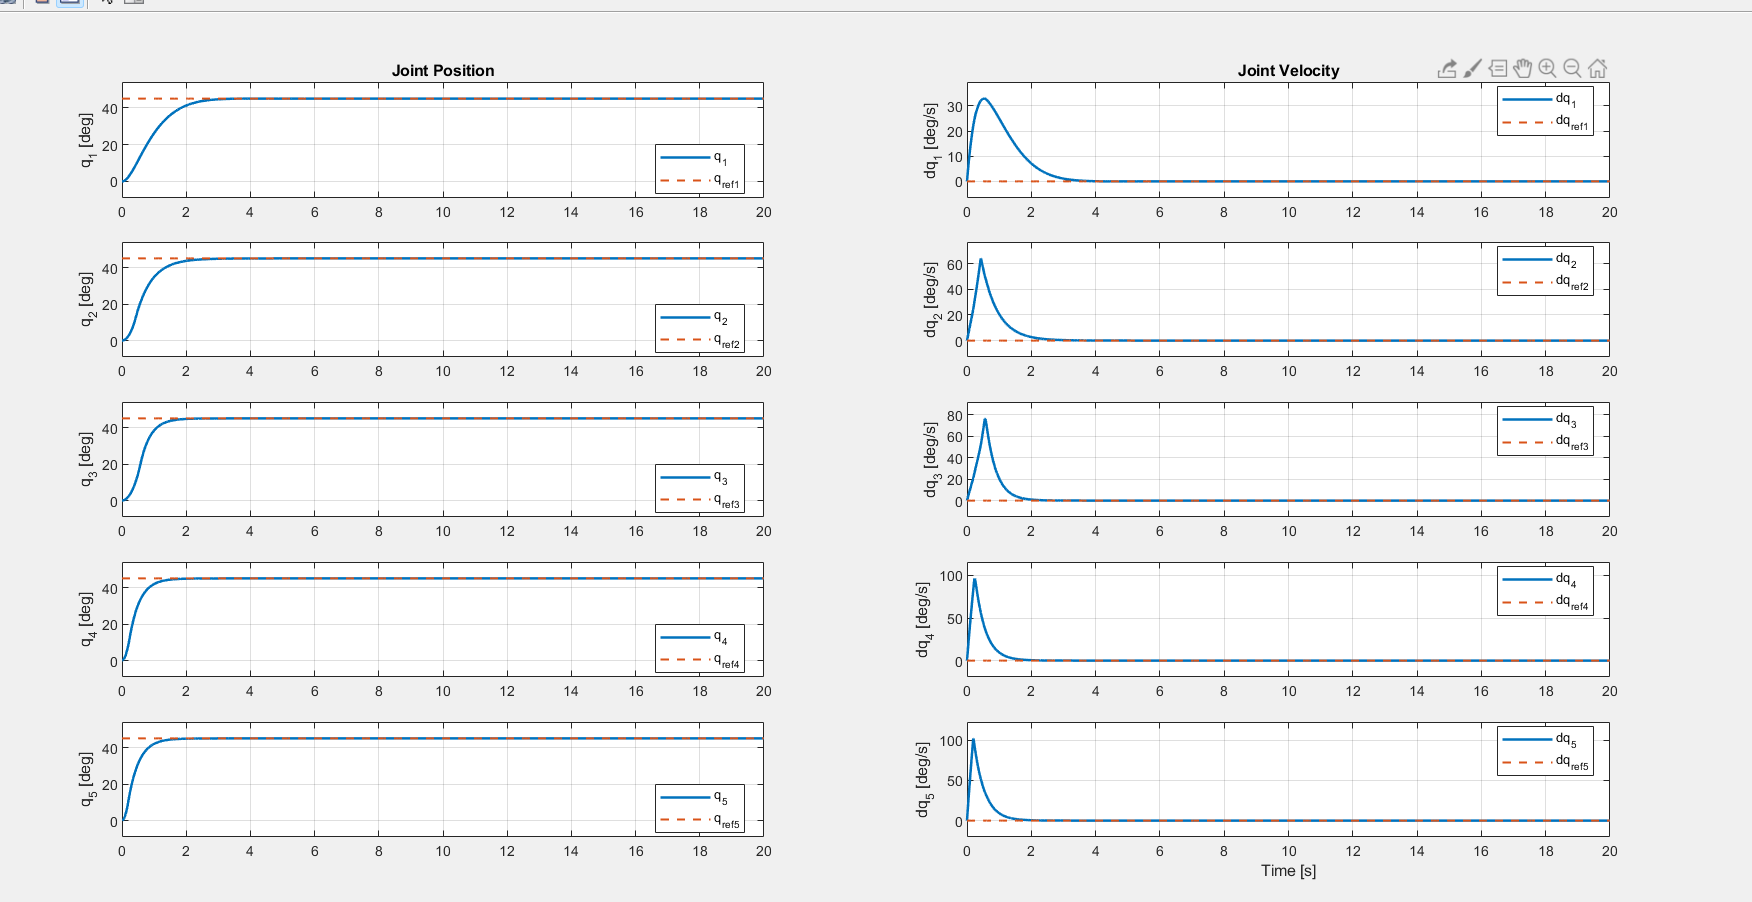
\includegraphics[width=\textwidth]{resources/images/PID_response}
    \caption{\centering{استجابة مواضع وسرعات مفاصل الذراع باستخدام متحكم \LR{PID} مع تعويض الجاذبية}}
    \label{fig:pid_response}
\end{figure}

يلاحظ من الشكل أن مواضع المفاصل تتجه نحو القيم المرجعية المطلوبة وتستقر حولها بدقة جيدة. كما تظهر السرعات بقيم مرتفعة نسبياً في بداية الحركة نتيجة الانتقال من الوضع الابتدائي إلى الوضع المرجعي، ثم تنخفض تدريجياً حتى تقترب من الصفر بعد استقرار المفاصل. يدل ذلك على أن المتحكم قادر على تحقيق تتبع جيد للموضع مع تخميد مناسب للحركة بعد الوصول إلى الوضع المطلوب.

تسمح هذه البنية بتحسين دقة تتبع الموضع مقارنة باستخدام متحكم \LR{PID} فقط، لأن حد تعويض الجاذبية يوفر جزءاً أساسياً من إشارة التحكم اللازمة لموازنة وزن الذراع، بينما يتولى متحكم \LR{PID} تصحيح خطأ التتبع وتحسين السلوك الانتقالي للنظام. وفي حال اختيار \(K_i=0\)، تتحول البنية عملياً إلى متحكم \LR{PD} مع تعويض الجاذبية، مع بقاء الصياغة العامة صالحة لمتحكم \LR{PID}.










%###############################################
%Adaptive
%###############################################


















\subsection{تطبيق التحكم التكيفي المعتمد على العزم المحسوب \LR{ACTC}}
\label{subsec:adaptive_computed_torque_control}

تعرف هذه الخوارزمية باسم التحكم التكيفي المعتمد على العزم المحسوب \LR{Adaptive Computed Torque Control (ACTC)}. بعد تطبيق متحكم \LR{PID} مع تعويض الجاذبية، تم الانتقال إلى خوارزمية تحكم أكثر ارتباطاً بالنموذج الديناميكي للذراع، حيث تعتمد هذه الخوارزمية على حساب عزم التحكم المطلوب لكل مفصل اعتماداً على النموذج الرياضي للنظام، ثم تعديل بعض معاملات هذا الحساب أثناء التشغيل بهدف تحسين التتبع والتعويض عن عدم دقة النموذج أو تغير بعض المؤثرات الديناميكية.

انطلاقاً من النموذج الديناميكي الذي تم اشتقاقه في الفصول السابقة، وبعد دمج تأثير نموذج المشغلات، يمكن كتابة معادلة حركة الذراع بالشكل:

\begin{equation}
\left(M(q)+K_a\right)\ddot{q}
=
K_u u
-
K_v\dot{q}
-
G(q)
\label{eq:actc_dynamic_model_voltage}
\end{equation}

حيث إن \(M(q)\) و \(G(q)\) يمثلان الحدود الديناميكية الناتجة عن نموذج الذراع الميكانيكي، بينما تمثل الحدود \(K_u\)، \(K_v\)، و \(K_a\) تأثير نموذج المشغلات المستخدم في هذا العمل. وبذلك يكون النموذج المستخدم في تصميم المتحكم امتداداً للنموذج الديناميكي السابق، وليس نموذجاً مستقلاً عنه.

لأجل تبسيط صياغة قانون التحكم، تعرف مصفوفة العطالة الفعالة كما يلي:

\begin{equation}
M_e(q)=M(q)+K_a
\label{eq:actc_effective_inertia}
\end{equation}

وبذلك تصبح معادلة الحركة:

\begin{equation}
M_e(q)\ddot{q}
=
K_u u
-
K_v\dot{q}
-
G(q)
\label{eq:actc_effective_model_voltage}
\end{equation}

وبما أن خوارزمية \LR{ACTC} تصمم أولاً على مستوى العزم، نعرف عزم التحكم المكافئ بالعلاقة:

\begin{equation}
\tau = K_u u
\label{eq:actc_torque_voltage_relation}
\end{equation}

وعندها يمكن كتابة النموذج المكافئ بالشكل:

\begin{equation}
M_e(q)\ddot{q}
+
K_v\dot{q}
+
G(q)
=
\tau
\label{eq:actc_mechanical_model}
\end{equation}


توضح هذه الصياغة أن عزم التحكم المطلوب يجب أن يعوض تأثير العطالة، وتأثير السرعة الناتج عن نموذج المشغلات، إضافة إلى عزوم الجاذبية. وبعد حساب عزم التحكم \(\tau\)، يتم تحويله لاحقاً إلى جهد مكافئ باستخدام العلاقة العكسية بين العزم والجهد.

تعتمد خوارزمية \LR{ACTC} على جعل الذراع يتتبع مساراً مرجعياً متدرجاً بدلاً من الانتقال المباشر إلى الموضع النهائي. لذلك تم استخدام نموذج مرجعي من الدرجة الثانية لتوليد الموضع والسرعة والتسارع المرجعيين لكل مفصل. يعطى النموذج المرجعي لكل مفصل بالعلاقة:

\begin{equation}
\ddot{q}_{m,i}
+
2\zeta_i\omega_{n,i}\dot{q}_{m,i}
+
\omega_{n,i}^{2}q_{m,i}
=
\omega_{n,i}^{2}q_{ref,i}
\label{eq:actc_reference_model_single_joint}
\end{equation}

حيث يمثل \(q_{ref,i}\) الموضع النهائي المطلوب للمفصل، بينما يمثل \(q_{m,i}\) الموضع المرجعي المتدرج الناتج عن النموذج المرجعي. وبذلك لا يتم تطبيق الانتقال إلى الموضع المطلوب بشكل مباشر، وإنما يتم توليد مسار ناعم يحاول النظام الحقيقي تتبعه.

يمكن كتابة النموذج المرجعي لجميع المفاصل بصيغة فضاء الحالة كما يلي:

\begin{equation}
\dot{x}_m=A_m x_m+B_m q_{ref}
\label{eq:actc_reference_state_space}
\end{equation}

حيث يعرف متجه حالة النموذج المرجعي بالعلاقة:

\begin{equation}
x_m=
\begin{bmatrix}
q_m\\
\dot{q}_m
\end{bmatrix}
\label{eq:actc_reference_state_vector}
\end{equation}

وتمثل \(q_m\) و \(\dot{q}_m\) على الترتيب الموضع والسرعة المرجعيين الناتجين عن النموذج المرجعي. أما مصفوفتا النموذج المرجعي فتكتبان بالشكل:

\begin{equation}
A_m=
\begin{bmatrix}
0_{5\times5} & I_{5\times5}\\
-\Omega_n^2 & -2Z\Omega_n
\end{bmatrix}
\label{eq:actc_Am_matrix}
\end{equation}

\begin{equation}
B_m=
\begin{bmatrix}
0_{5\times5}\\
\Omega_n^2
\end{bmatrix}
\label{eq:actc_Bm_matrix}
\end{equation}

حيث إن:

\begin{equation}
\Omega_n=
\mathrm{diag}
\left(
\omega_{n,1},
\omega_{n,2},
\omega_{n,3},
\omega_{n,4},
\omega_{n,5}
\right)
\label{eq:actc_omega_matrix}
\end{equation}

و:

\begin{equation}
Z=
\mathrm{diag}
\left(
\zeta_1,
\zeta_2,
\zeta_3,
\zeta_4,
\zeta_5
\right)
\label{eq:actc_zeta_matrix}
\end{equation}

بعد توليد المسار المرجعي، يتم تعريف خطأ الموضع بين الذراع الحقيقي والنموذج المرجعي كما يلي:

\begin{equation}
e=q-q_m
\label{eq:actc_position_error}
\end{equation}

كما يعرف خطأ السرعة بالعلاقة:

\begin{equation}
\dot{e}=\dot{q}-\dot{q}_m
\label{eq:actc_velocity_error}
\end{equation}

ولا يكتفي المتحكم باستخدام خطأ الموضع فقط، لأن الموضع قد يكون قريباً من المرجع بينما تكون السرعة غير مناسبة، كما لا يكفي استخدام خطأ السرعة فقط، لأن المفصل قد يتحرك بسرعة قريبة من السرعة المرجعية ولكنه ما يزال بعيداً عن الموضع المطلوب. لذلك يتم تعريف خطأ مركب يجمع بين خطأ الموضع وخطأ السرعة:

\begin{equation}
s=\dot{e}+\Lambda e
\label{eq:actc_composite_error}
\end{equation}

حيث تمثل \(\Lambda\) مصفوفة قطرية موجبة تحدد وزن خطأ الموضع داخل الخطأ المركب:

\begin{equation}
\Lambda=
\mathrm{diag}
\left(
\lambda_1,
\lambda_2,
\lambda_3,
\lambda_4,
\lambda_5
\right)
\label{eq:actc_lambda_matrix}
\end{equation}

إن الهدف من المتحكم هو جعل الخطأ المركب \(s\) يقترب من الصفر. فعندما يتحقق:

\begin{equation}
s=0
\label{eq:actc_composite_error_zero}
\end{equation}

نحصل على:

\begin{equation}
\dot{e}+\Lambda e=0
\label{eq:actc_error_dynamics}
\end{equation}

وبما أن \(\Lambda\) مصفوفة قطرية موجبة، فإن هذه المعادلة تؤدي إلى تناقص خطأ الموضع مع الزمن، أي:

\begin{equation}
e\rightarrow 0
\label{eq:actc_error_convergence}
\end{equation}

وبالتالي:

\begin{equation}
q\rightarrow q_m
\label{eq:actc_tracking_goal}
\end{equation}

بعد تعريف الخطأ المركب \(s\)، يتم تعريف تسارع مرجعي معدل يستخدم في حساب عزم التحكم. يكتب هذا التسارع بالعلاقة:

\begin{equation}
\ddot{q}_r=
\ddot{q}_m
-
\Lambda \dot{e}
\label{eq:actc_modified_reference_acceleration}
\end{equation}

حيث يمثل \(\ddot{q}_r\) التسارع المرجعي المعدل، وهو لا يساوي فقط تسارع النموذج المرجعي، بل يحتوي أيضاً على حد تصحيحي مرتبط بخطأ السرعة. والهدف من هذا التعريف هو ربط قانون التحكم مباشرة بالخطأ المركب \(s\).

وباشتقاق الخطأ المركب نحصل على:

\begin{equation}
\dot{s}
=
\ddot{e}
+
\Lambda\dot{e}
\label{eq:actc_s_derivative_1}
\end{equation}

وبما أن:

\begin{equation}
\ddot{e}
=
\ddot{q}
-
\ddot{q}_m
\label{eq:actc_acceleration_error}
\end{equation}

فإن:

\begin{equation}
\dot{s}
=
\ddot{q}
-
\ddot{q}_m
+
\Lambda\dot{e}
\label{eq:actc_s_derivative_2}
\end{equation}

وباستخدام تعريف \(\ddot{q}_r\)، يمكن كتابة:

\begin{equation}
\dot{s}
=
\ddot{q}
-
\ddot{q}_r
\label{eq:actc_s_derivative_final}
\end{equation}

توضح العلاقة السابقة أن تقليل الخطأ المركب \(s\) يرتبط بجعل تسارع الذراع الحقيقي \(\ddot{q}\) قريباً من التسارع المرجعي المعدل \(\ddot{q}_r\). لذلك يتم استخدام \(\ddot{q}_r\) داخل قانون العزم المحسوب.

في حال كان النموذج الديناميكي معروفاً بدقة، يمكن كتابة عزم التحكم المحسوب بالشكل:

\begin{equation}
\tau
=
M_e(q)\ddot{q}_r
+
K_v\dot{q}
+
G(q)
-
K_s s
\label{eq:actc_nominal_computed_torque}
\end{equation}

حيث تمثل \(K_s\) مصفوفة قطرية موجبة تستخدم لتخميد الخطأ المركب وتحسين استجابة النظام:

\begin{equation}
K_s=
\mathrm{diag}
\left(
k_{s1},
k_{s2},
k_{s3},
k_{s4},
k_{s5}
\right)
\label{eq:actc_Ks_matrix}
\end{equation}

إلا أن النموذج الديناميكي والمشغلات قد لا يكونان ممثلين بدقة كاملة، لذلك تم إدخال معاملات تكيفية تسمح بتعديل مساهمة حدود النموذج أثناء التشغيل. ولهذا الغرض يعرف شعاع النموذج لكل مفصل كما يلي:

\begin{equation}
Y_i
=
\begin{bmatrix}
\left(M_e(q)\ddot{q}_r\right)_i\\
\left(K_v\dot{q}\right)_i\\
G_i(q)\\
1
\end{bmatrix}
\label{eq:actc_regressor_vector}
\end{equation}

حيث يحتوي الشعاع \(Y_i\) على الحدود الأساسية المؤثرة في عزم المفصل \(i\)، وهي حد العطالة، وحد السرعة، وحد الجاذبية، إضافة إلى حد ثابت يستخدم للتعويض عن أي تأثير ثابت غير ممثل بدقة في النموذج.

ويعرف متجه المعاملات التكيفية لكل مفصل بالعلاقة:

\begin{equation}
\hat{\theta}_i
=
\begin{bmatrix}
\hat{\theta}_{M,i}\\
\hat{\theta}_{V,i}\\
\hat{\theta}_{G,i}\\
\hat{\theta}_{0,i}
\end{bmatrix}
\label{eq:actc_adaptive_parameters}
\end{equation}

حيث تمثل \(\hat{\theta}_{M,i}\) معامل تصحيح حد العطالة، وتمثل \(\hat{\theta}_{V,i}\) معامل تصحيح حد السرعة، وتمثل \(\hat{\theta}_{G,i}\) معامل تصحيح حد الجاذبية، بينما يمثل \(\hat{\theta}_{0,i}\) حداً ثابتاً للتعويض عن الانحيازات أو الأحمال غير الممثلة في النموذج.

بناءً على ذلك، يكتب قانون عزم التحكم التكيفي لكل مفصل كما يلي:

\begin{equation}
\tau_i
=
\hat{\theta}_i^{T}Y_i
-
K_{s,i}s_i
\label{eq:actc_adaptive_torque_single_joint}
\end{equation}
\begin{equation}
\begin{aligned}
\tau_i
=&\;
\hat{\theta}_{M,i}
\left(M_e(q)\ddot{q}_r\right)_i
+
\hat{\theta}_{V,i}
\left(K_v\dot{q}\right)_i
+
\hat{\theta}_{G,i}
G_i(q)
+
\hat{\theta}_{0,i}
-
K_{s,i}s_i
\end{aligned}
\label{eq:actc_adaptive_torque_expanded}
\end{equation}
وبصيغة عامة لجميع المفاصل، نحصل على متجه عزم التحكم:

\begin{equation}
\tau
=
\begin{bmatrix}
\tau_1\\
\tau_2\\
\tau_3\\
\tau_4\\
\tau_5
\end{bmatrix}
\label{eq:actc_adaptive_torque_vector}
\end{equation}

يمثل الحد \(\hat{\theta}_i^{T}Y_i\) الجزء المعتمد على النموذج الديناميكي، بينما يمثل الحد \(-K_{s,i}s_i\) جزءاً تصحيحياً مباشراً يعمل على تقليل الخطأ المركب. وبذلك لا يعتمد المتحكم فقط على النموذج الاسمي، بل يسمح بتعديل تأثير حد العطالة والسرعة والجاذبية أثناء التشغيل.

يتم تعديل معاملات المتحكم التكيفية أثناء التشغيل اعتماداً على قيمة الخطأ المركب \(s_i\) وشعاع النموذج \(Y_i\). ولهذا الغرض تم استخدام قانون تحديث من الشكل:

\begin{equation}
\dot{\hat{\theta}}_i
=
-
\frac{\Gamma Y_i s_i}{1+Y_i^{T}Y_i}
-
\sigma
\left(
\hat{\theta}_i-\theta_{nom}
\right)
\label{eq:actc_adaptation_law}
\end{equation}

حيث تمثل \(\Gamma\) مصفوفة كسب التكيف، وهي مصفوفة قطرية موجبة تحدد سرعة تعديل معاملات المتحكم:

\begin{equation}
\Gamma=
\mathrm{diag}
\left(
\gamma_M,
\gamma_V,
\gamma_G,
\gamma_0
\right)
\label{eq:actc_gamma_matrix}
\end{equation}

أما \(\theta_{nom}\) فيمثل متجه القيم الاسمية لمعاملات النموذج، وقد تم اختياره بالشكل:

\begin{equation}
\theta_{nom}
=
\begin{bmatrix}
1\\
1\\
1\\
0
\end{bmatrix}
\label{eq:actc_nominal_theta}
\end{equation}

تمثل القيم الثلاث الأولى معاملات اسمية لحدود العطالة والسرعة والجاذبية، بينما يمثل العنصر الرابع قيمة اسمية للحد الثابت. وبذلك يبدأ المتحكم من النموذج الاسمي، ثم يقوم بتعديل مساهمة كل حد حسب خطأ التتبع الناتج أثناء الحركة.

يحتوي قانون التحديث أيضاً على الحد:

\begin{equation}
-
\sigma
\left(
\hat{\theta}_i-\theta_{nom}
\right)
\label{eq:actc_sigma_modification}
\end{equation}

وهو ما يعرف باسم \LR{Sigma Modification}. يهدف هذا الحد إلى منع انجراف معاملات التكيف بعيداً عن القيم الاسمية، وخاصة عند وجود تشبع في إشارة التحكم أو عند وجود اضطرابات وضجيج في القياسات. وبذلك يساعد على جعل عملية التكيف أكثر استقراراً من الناحية العددية.

بعد حساب عزم التحكم التكيفي لكل مفصل، يتم تجميع عزوم المفاصل في المتجه:

\begin{equation}
\tau
=
\begin{bmatrix}
\tau_1&
\tau_2&
\tau_3&
\tau_4&
\tau_5
\end{bmatrix}^{T}
\label{eq:actc_control_torque_vector}
\end{equation}

وبما أن نموذج النظام المستخدم في المحاكاة يستقبل الجهد المكافئ \(u\) وليس العزم مباشرة، يتم تحويل عزم التحكم إلى جهد باستخدام العلاقة:

\begin{equation}
u_{raw}
=
K_u^{-1}\tau
\label{eq:actc_raw_voltage}
\end{equation}

حيث يمثل \(u_{raw}\) الجهد المطلوب قبل تطبيق حدود المشغلات. ونظراً لأن الجهد المسموح للمشغلات محدود فيزيائياً، يتم تطبيق حد تشبع على إشارة التحكم بحيث تبقى ضمن المجال:

\begin{equation}
-6 \leq u_i \leq 6
\label{eq:actc_voltage_limits}
\end{equation}

لذلك تكتب إشارة التحكم الفعلية بالشكل:

\begin{equation}
u_{sat}
=
\mathrm{sat}
\left(
u_{raw},-6,6
\right)
\label{eq:actc_saturated_voltage}
\end{equation}

وتعرف دالة التشبع لكل مفصل كما يلي:

\begin{equation}
u_{sat,i}
=
\begin{cases}
6, & u_{raw,i}>6\\
u_{raw,i}, & -6 \leq u_{raw,i} \leq 6\\
-6, & u_{raw,i}<-6
\end{cases}
\label{eq:actc_saturation_function}
\end{equation}

بعد تطبيق التشبع، يتم إدخال الجهد الناتج إلى النموذج الديناميكي المغلق للذراع. وبالاعتماد على معادلة الحركة المستخدمة، يحسب تسارع المفاصل من العلاقة:

\begin{equation}
\ddot{q}
=
\left(M(q)+K_a\right)^{-1}
\left(
K_u u_{sat}
-
K_v\dot{q}
-
G(q)
\right)
\label{eq:actc_closed_loop_acceleration}
\end{equation}

وبذلك يصبح النظام المغلق الناتج عن تطبيق خوارزمية \LR{ACTC} مع حدود الجهد كما يلي:

\begin{equation}
\ddot{q}
=
\left(M(q)+K_a\right)^{-1}
\left(
K_u u_{sat}
-
K_v\dot{q}
-
G(q)
\right)
\label{eq:actc_state_ddq}
\end{equation}

\begin{equation}
\dot{x}_m
=
A_m x_m+B_m q_{ref}
\label{eq:actc_state_reference_model}
\end{equation}

\begin{equation}
\dot{\hat{\theta}}_i
=
-
\frac{\Gamma Y_i s_i}{1+Y_i^{T}Y_i}
-
\sigma
\left(
\hat{\theta}_i-\theta_{nom}
\right)
\label{eq:actc_state_theta_dot}
\end{equation}

تم تنفيذ هذه المعادلات عددياً في بيئة \LR{MATLAB}، حيث تم حل النظام التفاضلي غير الخطي بعد تعريف المواضع الابتدائية، والنموذج المرجعي، ومصفوفات الكسب، ومعاملات التكيف. وتم استخراج مواضع المفاصل وسرعاتها وإشارات التحكم الناتجة بهدف تقييم أداء الخوارزمية في تتبع المسار المرجعي.


تم اختبار خوارزمية \LR{ACTC} باستخدام المواضع المرجعية نفسها المعتمدة في اختبار المتحكم السابق، وذلك من أجل تقييم قدرة الخوارزمية على تتبع المسار المرجعي المتدرج الناتج عن النموذج المرجعي. يوضح الشكل \ref{fig:adaptive_response} استجابة مواضع وسرعات مفاصل الذراع عند تطبيق خوارزمية التحكم التكيفي المعتمد على العزم المحسوب.

\begin{figure}[H]
    \centering
    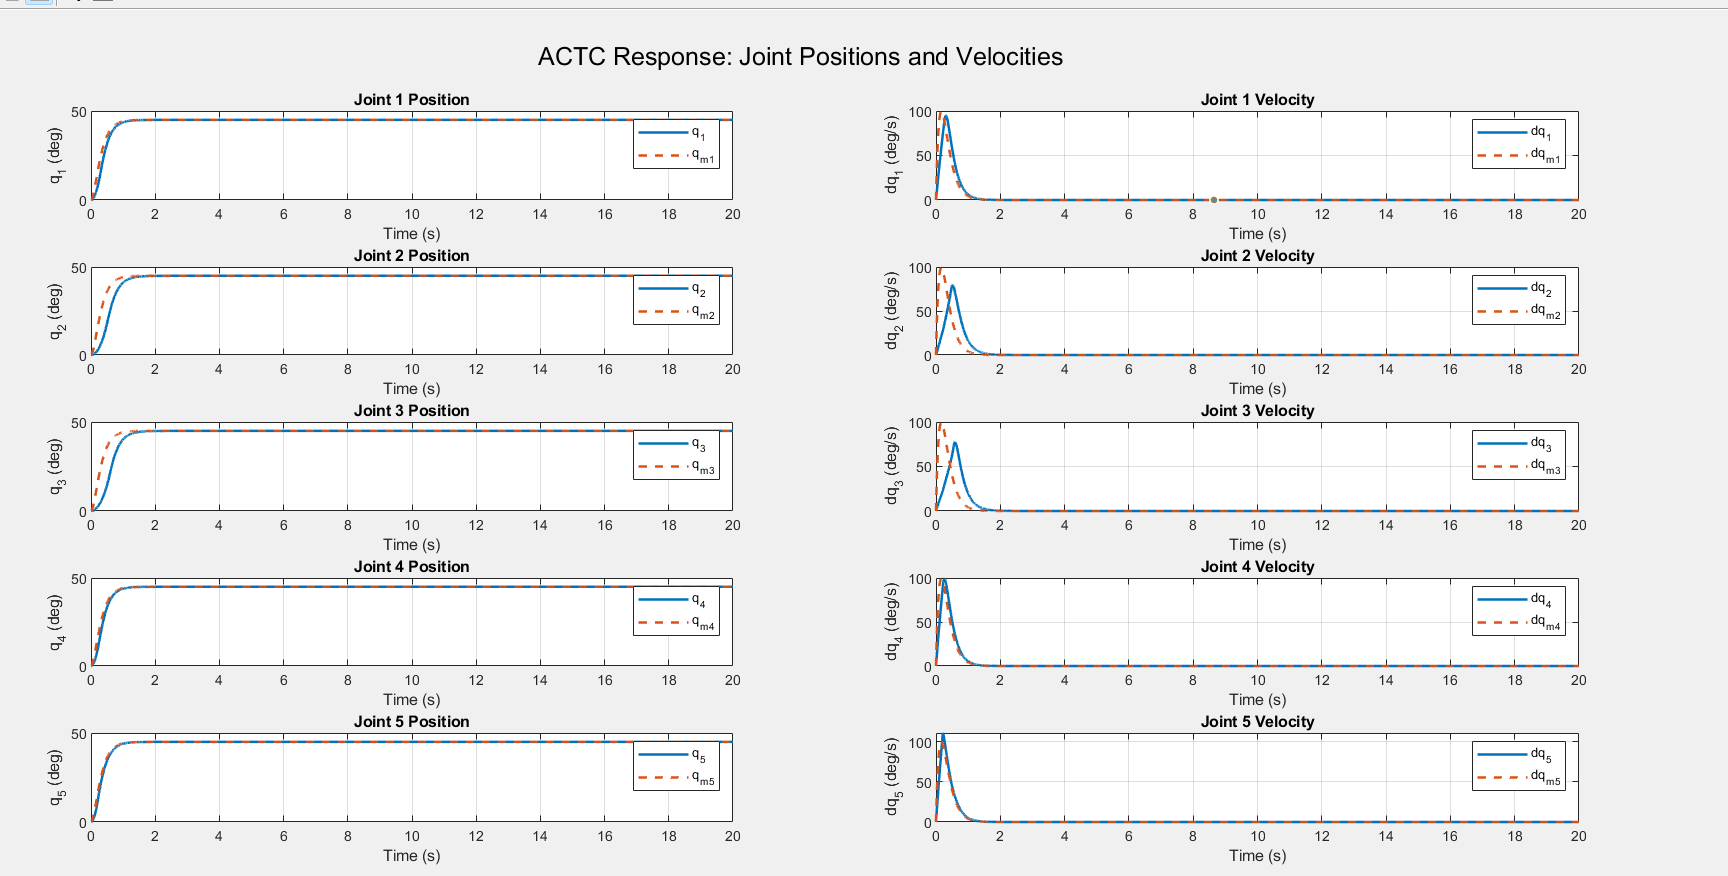
\includegraphics[width=\textwidth]{resources/images/Adaptive_response}
    \caption{\centering{استجابة مواضع وسرعات مفاصل الذراع باستخدام خوارزمية التحكم التكيفي المعتمد على العزم المحسوب \LR{ACTC}}}
    \label{fig:adaptive_response}
\end{figure}

يلاحظ من الشكل أن مواضع المفاصل تتبع المسارات المرجعية الناتجة عن النموذج المرجعي بصورة جيدة، حيث تتقارب الاستجابة الحقيقية مع الاستجابة المرجعية بعد فترة انتقالية قصيرة. كما تظهر السرعات بقيم مرتفعة في بداية الحركة نتيجة الانتقال من الوضع الابتدائي إلى الموضع المطلوب، ثم تنخفض تدريجياً حتى تقترب من الصفر بعد استقرار المفاصل.

تظهر فروقات نسبية في استجابة بعض المفاصل، وخصوصاً المفصلين الثاني والثالث، ويعود ذلك إلى أن هذين المفصلين يتحملان جزءاً أكبر من حمل الذراع، مما يزيد من تأثير العطالة والجاذبية عليهما. ومع ذلك، فإن الخوارزمية استطاعت تحقيق تتبع مقبول للمسارات المرجعية دون ظهور اهتزازات واضحة أو خطأ دائم كبير في الموضع.

تبيّن هذه النتيجة أن استخدام النموذج الديناميكي ضمن قانون التحكم، مع تعديل معاملات العطالة والسرعة والجاذبية بشكل تكيفي، يساعد على تحسين قدرة المتحكم على تتبع المسار المرجعي مقارنة بالاعتماد على تصحيح الخطأ فقط.

















%###############################################
%Sliding Mode Control
%###############################################


























\subsection{تطبيق التحكم الانزلاقي \LR{SMC}}
\label{subsec:sliding_mode_control}

تعرف هذه الخوارزمية باسم التحكم الانزلاقي \LR{Sliding Mode Control (SMC)}. وهي من خوارزميات التحكم القوية المستخدمة مع الأنظمة غير الخطية، إذ تعتمد على دفع حالة النظام نحو سطح محدد يسمى سطح الانزلاق، ثم إبقاء حركة النظام قريبة من هذا السطح. وعند تحقق ذلك، يتناقص خطأ التتبع تدريجياً باتجاه الصفر.

كما في الخوارزميات السابقة، تم الانطلاق من النموذج الديناميكي بعد دمج تأثير المشغلات:

\begin{equation}
\left(M(q)+K_a\right)\ddot{q}
=
K_u u
-
K_v\dot{q}
-
G(q)
\label{eq:smc_dynamic_model_voltage}
\end{equation}

وبتعريف مصفوفة العطالة الفعالة:

\begin{equation}
M_e(q)=M(q)+K_a
\label{eq:smc_effective_inertia}
\end{equation}

وباعتبار أن عزم التحكم المكافئ الناتج عن الجهد هو:

\begin{equation}
\tau=K_u u
\label{eq:smc_torque_voltage_relation}
\end{equation}

يمكن كتابة النموذج على مستوى العزم كما يلي:

\begin{equation}
M_e(q)\ddot{q}
+
K_v\dot{q}
+
G(q)
=
\tau
\label{eq:smc_mechanical_model}
\end{equation}

تجدر الإشارة إلى أن خوارزمية التحكم الانزلاقي لا تتطلب نموذجاً مرجعياً بحد ذاته، وإنما تحتاج إلى مسار مطلوب \(q_d(t)\) مع مشتقاته \(\dot{q}_d(t)\) و \(\ddot{q}_d(t)\). وفي هذا العمل تم استخدام المسار المرجعي المتدرج نفسه المستخدم في خوارزمية \LR{ACTC}، وذلك من أجل جعل المقارنة بين الخوارزميات أكثر اتساقاً. لذلك تم اختيار:

\begin{equation}
q_d=q_m,
\qquad
\dot{q}_d=\dot{q}_m,
\qquad
\ddot{q}_d=\ddot{q}_m
\label{eq:smc_reference_choice}
\end{equation}

يعرف خطأ الموضع بالعلاقة:

\begin{equation}
e=q-q_d
\label{eq:smc_position_error}
\end{equation}

كما يعرف خطأ السرعة كما يلي:

\begin{equation}
\dot{e}=\dot{q}-\dot{q}_d
\label{eq:smc_velocity_error}
\end{equation}

بعد ذلك يتم تعريف سطح الانزلاق بالعلاقة:

\begin{equation}
s=\dot{e}+\Lambda e
\label{eq:smc_sliding_surface}
\end{equation}

حيث تمثل \(\Lambda\) مصفوفة قطرية موجبة:

\begin{equation}
\Lambda=
\mathrm{diag}
\left(
\lambda_1,
\lambda_2,
\lambda_3,
\lambda_4,
\lambda_5
\right)
\label{eq:smc_lambda_matrix}
\end{equation}

يمثل الشرط \(s=0\) سطح الانزلاق المطلوب. فعند تحقق هذا الشرط نحصل على:

\begin{equation}
\dot{e}+\Lambda e=0
\label{eq:smc_error_dynamics}
\end{equation}

وبما أن \(\Lambda\) موجبة، فإن هذه المعادلة تؤدي إلى تناقص خطأ الموضع مع الزمن، أي:

\begin{equation}
e\rightarrow 0
\label{eq:smc_error_convergence}
\end{equation}

وبالتالي يتحقق تتبع المسار المطلوب:

\begin{equation}
q\rightarrow q_d
\label{eq:smc_tracking_goal}
\end{equation}

كما في الخوارزمية السابقة، يتم تعريف تسارع مرجعي معدل بالعلاقة:

\begin{equation}
\ddot{q}_r=
\ddot{q}_d
-
\Lambda\dot{e}
\label{eq:smc_modified_reference_acceleration}
\end{equation}

وباستخدام هذا التعريف يمكن ربط مشتق سطح الانزلاق بتسارع الذراع الحقيقي، إذ إن:

\begin{equation}
\dot{s}
=
\ddot{e}
+
\Lambda\dot{e}
\label{eq:smc_s_derivative_1}
\end{equation}

وبما أن:

\begin{equation}
\ddot{e}
=
\ddot{q}
-
\ddot{q}_d
\label{eq:smc_acceleration_error}
\end{equation}

فإن:

\begin{equation}
\dot{s}
=
\ddot{q}
-
\ddot{q}_d
+
\Lambda\dot{e}
\label{eq:smc_s_derivative_2}
\end{equation}

وباستخدام تعريف \(\ddot{q}_r\)، نحصل على:

\begin{equation}
\dot{s}
=
\ddot{q}
-
\ddot{q}_r
\label{eq:smc_s_derivative_final}
\end{equation}

توضح هذه العلاقة أن جعل تسارع الذراع الحقيقي قريباً من \(\ddot{q}_r\) يساعد على تقليل سطح الانزلاق \(s\)، وبالتالي تقليل خطأ التتبع.

يعطى قانون عزم التحكم الانزلاقي المستخدم في هذا العمل بالعلاقة:

\begin{equation}
\tau
=
M_e(q)\ddot{q}_r
+
K_v\dot{q}
+
G(q)
-
K_s s
-
K_r
\mathrm{sat}
\left(
\frac{s}{\varepsilon}
\right)
\label{eq:smc_control_law}
\end{equation}

حيث تمثل \(K_s\) مصفوفة قطرية موجبة تستخدم لتوليد تصحيح ناعم للخطأ المركب:

\begin{equation}
K_s=
\mathrm{diag}
\left(
k_{s1},
k_{s2},
k_{s3},
k_{s4},
k_{s5}
\right)
\label{eq:smc_Ks_matrix}
\end{equation}

أما \(K_r\) فهي مصفوفة قطرية موجبة تمثل كسب الحد الانزلاقي القوي:

\begin{equation}
K_r=
\mathrm{diag}
\left(
k_{r1},
k_{r2},
k_{r3},
k_{r4},
k_{r5}
\right)
\label{eq:smc_Kr_matrix}
\end{equation}

يمثل الحد:

\begin{equation}
-
K_r
\mathrm{sat}
\left(
\frac{s}{\varepsilon}
\right)
\label{eq:smc_robust_term}
\end{equation}

الجزء الأساسي الذي يميز التحكم الانزلاقي، إذ يعمل على دفع النظام باتجاه سطح الانزلاق \(s=0\). وفي الصياغة النظرية المثالية يمكن استخدام دالة الإشارة \(\mathrm{sign}(s)\)، إلا أن استخدامها قد يؤدي إلى اهتزازات سريعة في إشارة التحكم تعرف باسم \LR{Chattering}. لذلك تم استخدام دالة التشبع \(\mathrm{sat}\) بدلاً منها، بهدف تقليل هذه الاهتزازات.

تعرف دالة التشبع كما يلي:

\begin{equation}
\mathrm{sat}(x)
=
\begin{cases}
1, & x>1\\
x, & -1 \leq x \leq 1\\
-1, & x<-1
\end{cases}
\label{eq:smc_saturation_function}
\end{equation}

أما \(\varepsilon\) فتمثل عرض الطبقة الحدودية \LR{Boundary Layer}. عندما تكون قيمة \(s\) كبيرة، يعمل الحد الانزلاقي بقوة باتجاه تقليل الخطأ، وعندما يقترب \(s\) من الصفر تصبح دالة التشبع أكثر نعومة، مما يساعد على تخفيف الاهتزاز في إشارة التحكم.

بعد حساب عزم التحكم \(\tau\)، يتم تحويله إلى جهد مكافئ كما في الخوارزميات السابقة:

\begin{equation}
u_{raw}
=
K_u^{-1}\tau
\label{eq:smc_raw_voltage}
\end{equation}

ونظراً لأن الجهد المسموح للمشغلات محدود فيزيائياً، يتم تطبيق حد التشبع:

\begin{equation}
-6 \leq u_i \leq 6
\label{eq:smc_voltage_limits}
\end{equation}

لذلك تكون إشارة التحكم الفعلية:

\begin{equation}
u_{sat}
=
\mathrm{sat}
\left(
u_{raw},-6,6
\right)
\label{eq:smc_saturated_voltage}
\end{equation}

بعد ذلك يدخل الجهد المشبع إلى النموذج الديناميكي، ويحسب تسارع المفاصل من العلاقة:

\begin{equation}
\ddot{q}
=
\left(M(q)+K_a\right)^{-1}
\left(
K_u u_{sat}
-
K_v\dot{q}
-
G(q)
\right)
\label{eq:smc_closed_loop_acceleration}
\end{equation}

تم تنفيذ خوارزمية \LR{SMC} عددياً في بيئة \LR{MATLAB} باستخدام المسار المرجعي نفسه المستخدم في خوارزمية \LR{ACTC}. يوضح الشكل \ref{fig:sliding_mode_response} استجابة مواضع وسرعات مفاصل الذراع عند تطبيق التحكم الانزلاقي.

\begin{figure}[H]
    \centering
    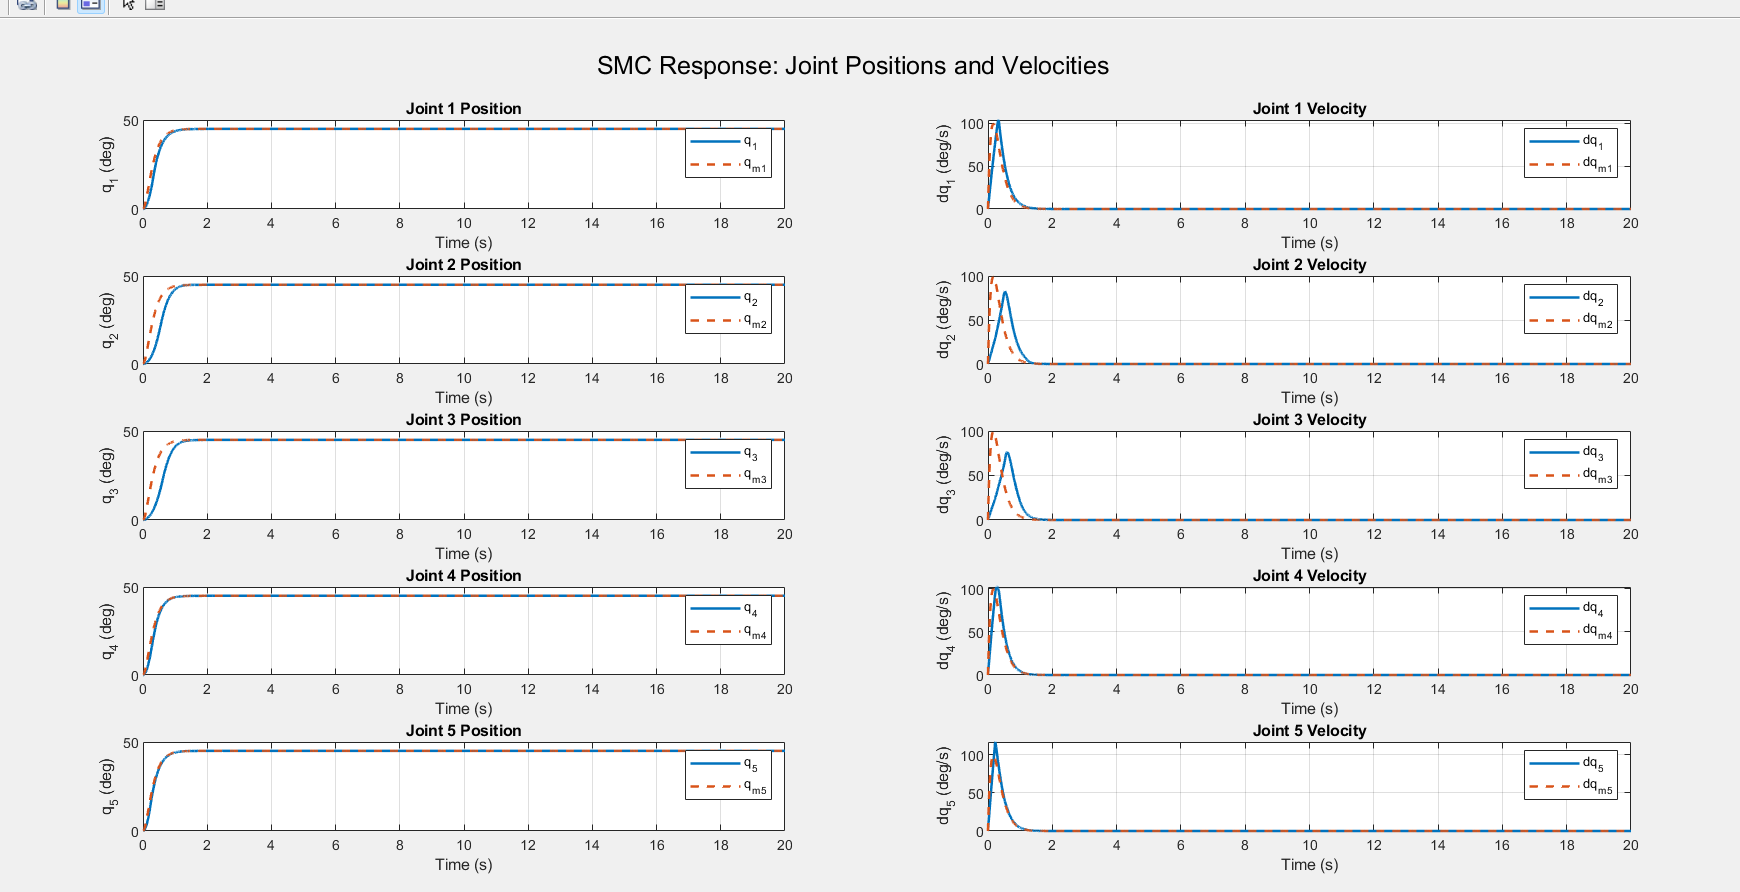
\includegraphics[width=\textwidth]{resources/images/Sliding_mode_response}
    \caption{\centering{استجابة مواضع وسرعات مفاصل الذراع باستخدام خوارزمية التحكم الانزلاقي \LR{SMC}}}
    \label{fig:sliding_mode_response}
\end{figure}

يلاحظ من الشكل أن خوارزمية \LR{SMC} استطاعت تحقيق تتبع جيد للمسارات المرجعية، إذ تقترب مواضع المفاصل الحقيقية من المواضع المرجعية وتستقر عند القيم المطلوبة. كما تظهر السرعات بقيم مرتفعة في بداية الحركة نتيجة الانتقال من الوضع الابتدائي إلى المسار المرجعي، ثم تتناقص تدريجياً حتى تقترب من الصفر بعد استقرار المفاصل.

تظهر استجابة المفصلين الثاني والثالث أبطأ نسبياً مقارنة ببعض المفاصل الأخرى، ويعود ذلك إلى تأثير الحمل الأكبر الواقع عليهما ضمن بنية الذراع. كما أن حدود التشبع المفروضة على الجهد تلعب دوراً مهماً في تحديد سرعة التتبع، لأن المشغلات لا تستطيع تطبيق جهد أكبر من المجال الفيزيائي المسموح. ومع ذلك، فإن الاستجابة العامة تبقى مستقرة ودون اهتزازات واضحة في الموضع، مما يدل على قدرة التحكم الانزلاقي على دفع النظام نحو سطح الانزلاق وتحقيق تتبع مقبول للمسار المرجعي.















\subsection{تحليل ومقارنة أداء خوارزميات التحكم}
\label{subsec:controllers_comparison}

بعد تطبيق خوارزميات التحكم الثلاث، وهي متحكم \LR{PID} مع تعويض الجاذبية، والتحكم التكيفي المعتمد على العزم المحسوب \LR{ACTC}، والتحكم الانزلاقي \LR{SMC}، تم إجراء مقارنة بين الاستجابات الناتجة اعتماداً على مواضع وسرعات المفاصل. ولجعل المقارنة أكثر وضوحاً، تم عرض استجابات الخوارزميات الثلاث ضمن الشكل نفسه، كما هو مبين في الشكل \ref{fig:comparison_actc_pid_smc}.

\begin{figure}[H]
    \centering
    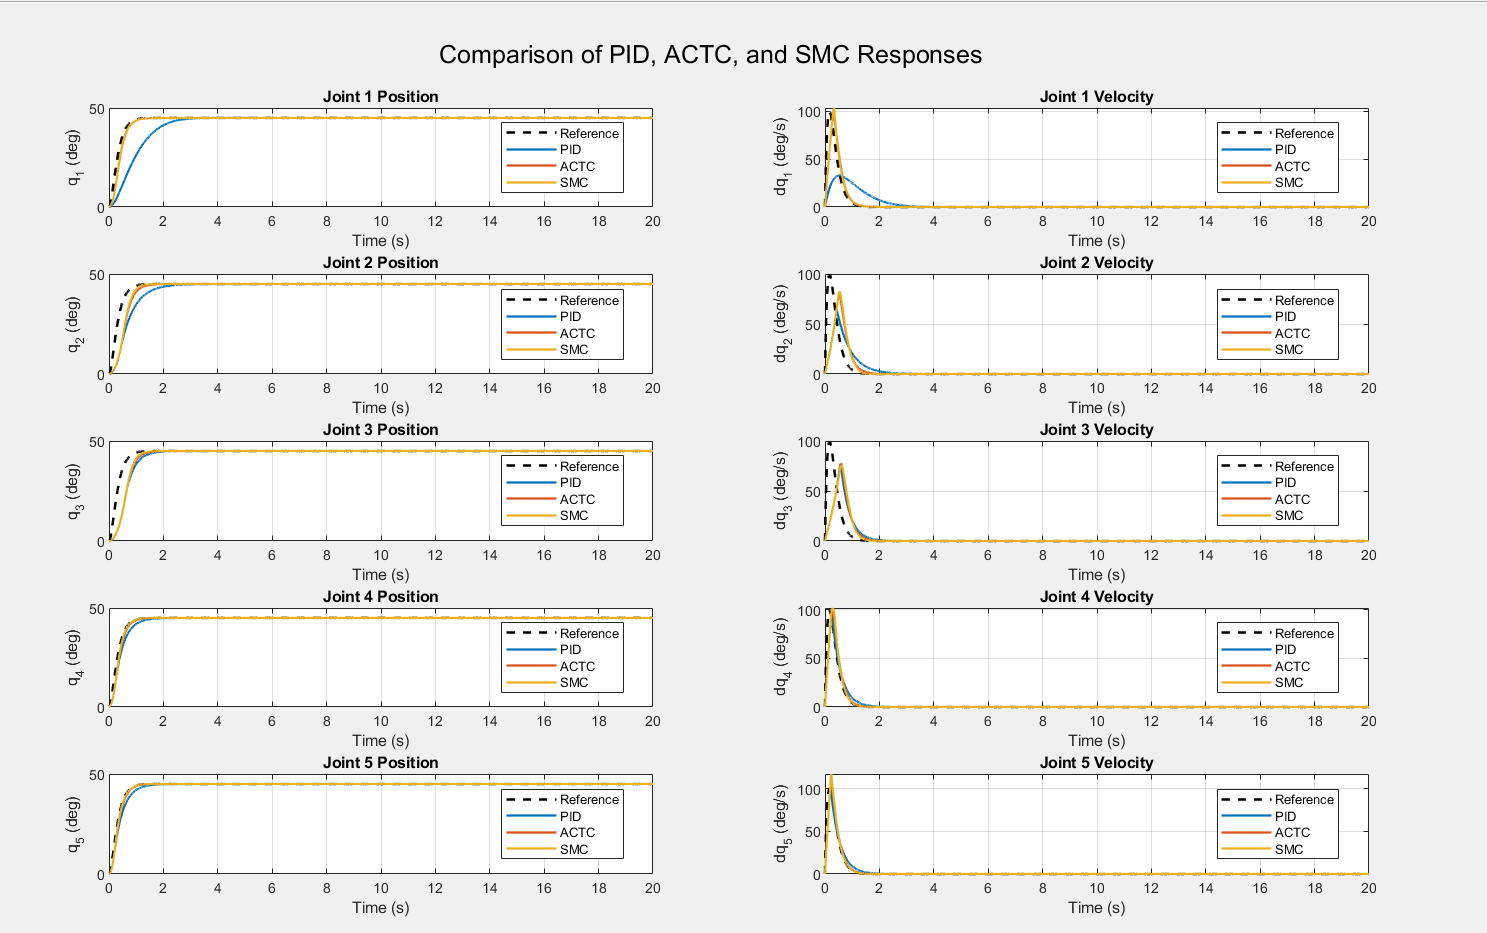
\includegraphics[width=\textwidth]{resources/images/Comparison_ACTC_PID_SMC}
    \caption{\centering{مقارنة استجابات مواضع وسرعات المفاصل باستخدام خوارزميات \LR{PID} و \LR{ACTC} و \LR{SMC}}}
    \label{fig:comparison_actc_pid_smc}
\end{figure}

يوضح الشكل \ref{fig:comparison_actc_pid_smc} أن الخوارزميات الثلاث قادرة على تحقيق تتبع مقبول للمسارات المرجعية، مع وجود اختلافات في سرعة الاستجابة وشكل السرعات الناتجة. ويُلاحظ أن متحكم \LR{PID} مع تعويض الجاذبية يمثل الحل الأبسط من حيث البنية والضبط، بينما تعتمد خوارزميتا \LR{ACTC} و \LR{SMC} على النموذج الديناميكي بصورة أوضح.


\small
\renewcommand{\arraystretch}{1.5}

\begin{longtable}{|p{3.2cm}|p{3.6cm}|p{3.6cm}|p{3.6cm}|}
\caption{مقارنة أداء خوارزميات التحكم المطبقة}
\label{tab:controllers_comparison}\\

\hline
\centering المعيار
&
\centering \LR{PID} مع تعويض الجاذبية
&
\centering \LR{ACTC}
&
\centering \LR{SMC}
\tabularnewline
\hline
\endfirsthead

\hline
\centering المعيار
&
\centering \LR{PID} مع تعويض الجاذبية
&
\centering \LR{ACTC}
&
\centering \LR{SMC}
\tabularnewline
\hline
\endhead

مبدأ العمل
&
يعتمد على خطأ الموضع والسرعة مع إضافة تعويض مباشر للجاذبية.
&
يعتمد على النموذج الديناميكي مع تعديل معاملات العطالة والسرعة والجاذبية أثناء التشغيل.
&
يعتمد على دفع النظام نحو سطح الانزلاق \(s=0\) باستخدام حد قوي مقاوم للخطأ.
\tabularnewline
\hline

الاعتماد على النموذج
&
اعتماد محدود، حيث يستخدم النموذج أساساً لتعويض الجاذبية.
&
اعتماد واضح على النموذج الديناميكي، مع قدرة على تعديل مساهمة حدوده أثناء التشغيل.
&
اعتماد واضح على النموذج مع إضافة حد انزلاقي لتحسين المتانة.
\tabularnewline
\hline

التعامل مع تغيرات النظام
&
محدود، لأنه لا يغير بنيته عند تغير الحمل أو خصائص الذراع.
&
الأفضل في هذه النقطة، لأنه يستطيع تعديل معاملات النموذج عند تغير الحمل أو إضافة وزن على الذراع.
&
يمتلك متانة جيدة ضد الاضطرابات، لكنه لا يعدل معاملات النموذج كما في \LR{ACTC}.
\tabularnewline
\hline

جودة تتبع الموضع
&
جيدة، خصوصاً بعد إضافة تعويض الجاذبية.
&
جيدة، مع أفضلية عند تغير خصائص النموذج الديناميكي.
&
جيدة ومستقرة، مع قدرة على دفع الخطأ نحو سطح الانزلاق.
\tabularnewline
\hline

استجابة السرعة
&
تظهر سرعة عالية في بداية الحركة ثم تتناقص بعد الاستقرار.
&
استجابة ناعمة نسبياً وتتبع جيد للسرعات المرجعية.
&
استجابة مستقرة، وقد تصبح أكثر حدة حسب قيم \(K_r\) و \(\varepsilon\).
\tabularnewline
\hline

تأثير التشبع
&
يتأثر بحدود الجهد، خصوصاً عند زيادة الكسب أو الحمل.
&
يتأثر أيضاً بالتشبع، خاصة في المفاصل التي تحتاج عزماً أكبر.
&
يتأثر بالتشبع كذلك، لأن الحد الانزلاقي قد يطلب جهداً أعلى من قدرة المشغلات.
\tabularnewline
\hline

سهولة الضبط
&
الأبسط من حيث الضبط والتنفيذ.
&
أعقد بسبب وجود معاملات التكيف وقانون التحديث.
&
متوسط إلى معقد بسبب اختيار \(K_s\)، و \(K_r\)، و \(\varepsilon\).
\tabularnewline
\hline

الملاحظة العامة
&
مناسب كبداية ويعطي أداء جيداً مع تعويض الجاذبية.
&
الأفضل عند احتمال تغير النموذج أو تغير الحمل، لأنه يمتلك قدرة تكيفية مع الحدود الديناميكية.
&
يعطي استجابة قوية ومستقرة، لكنه يحتاج ضبطاً مناسباً لتجنب الحدة أو الاهتزاز.
\tabularnewline
\hline

\end{longtable}

\normalsize

من خلال المقارنة، يتضح أن متحكم \LR{PID} مع تعويض الجاذبية يمثل الحل الأبسط والأقل تعقيداً، وقد استطاع تحقيق تتبع جيد للموضع. أما خوارزمية \LR{ACTC} فتظهر أهميتها عند تغير خصائص النظام الديناميكية، مثل حمل الذراع لوزن إضافي أو تغير تأثيرات العطالة والجاذبية، لأنها لا تعتمد فقط على تصحيح الخطأ، بل تقوم بتعديل معاملات النموذج أثناء التشغيل. لذلك تعد \LR{ACTC} أكثر ملاءمة للحالات التي قد يتغير فيها الحمل أو لا تكون معاملات النموذج معروفة بدقة كاملة. في المقابل، أظهرت خوارزمية \LR{SMC} استجابة مستقرة وقادرة على دفع النظام نحو سطح الانزلاق، لكنها لا تمتلك آلية تعلم مباشرة لمعاملات النموذج كما في الخوارزمية التكيفية.

ومع ذلك، فإن جميع الخوارزميات تبقى مقيدة بحدود الجهد المفروضة على المشغلات. لذلك فإن ظهور فروقات في التتبع، خاصة في المفصلين الثاني والثالث، لا يعود فقط إلى بنية المتحكم، بل يرتبط أيضاً بالقدرة الفيزيائية المحدودة للمحركات وبالعزوم الأكبر المطلوبة للتغلب على تأثير الجاذبية والعطالة في هذه المفاصل.








